\chapter{Scyther Scripts}
\label{app:listings}


\section{Adaptable Pairwise Key Establishment Scheme (APKES)}
\label{app:apkes}

\lstinputlisting{scripts/apkes.spdl}

\section{Adaptable Key Establishment Scheme (AKES)}
\label{app:akes}

\lstinputlisting{scripts/akes.spdl}

\newpage

\section{Secure Authentication and Key Establishment Scheme (SAKES)}
\label{app:sakes}

\subsection{SAKES - Authentication}
\label{app:sakes-auth}
\lstinputlisting{scripts/sakes-auth.spdl}

\newpage

\subsection{SAKES - Key Establishment}
\label{app:sakes-keys}
\lstinputlisting{scripts/sakes-keys.spdl}


\subsection{SAKES - Key Establishment - Interaction Between A and B}
\label{app:sakes-keys-ab}
\lstinputlisting{scripts/sakes-keys-ab.spdl}

\section{Secure Authentication and Key Establishment Scheme (SAKES) --- Improved}
\label{app:sakes-fixed-auth}
\lstinputlisting{scripts/fix/sakes-auth-fix.spdl}

\chapter{Attacks}
\label{app:attacks}

\begin{sidewaysfigure}
	\centering
	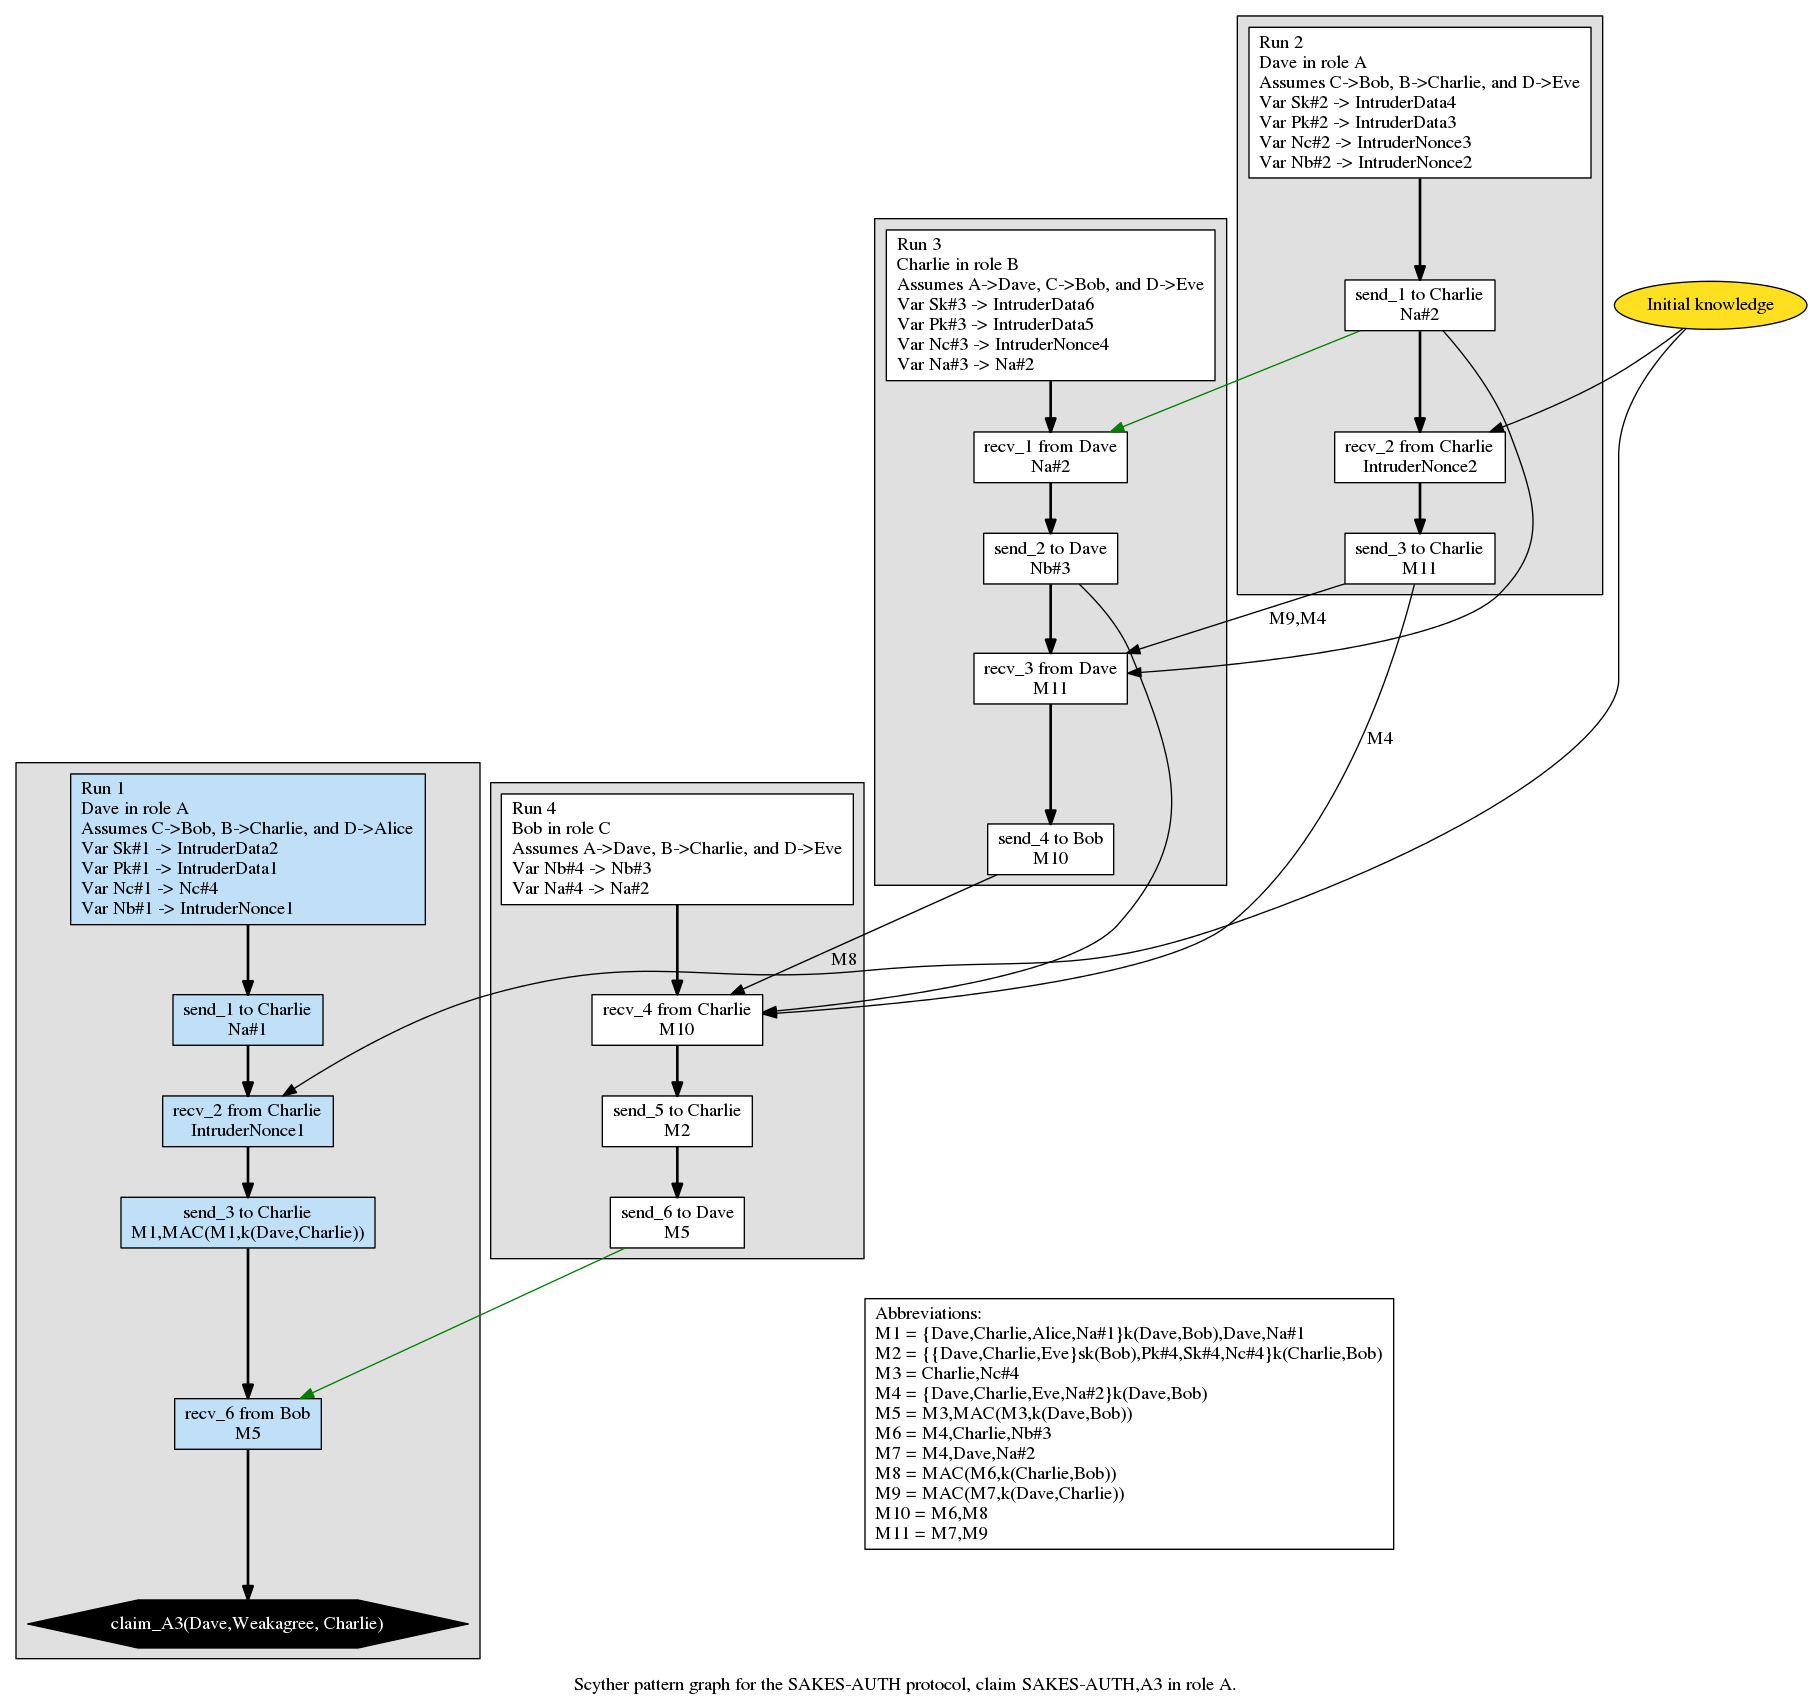
\includegraphics[scale=0.20]{attacks/sakes-auth-a-weakagree-attack2.png}
	\caption{Graph of the attack discovered on the Weakagree property of the role A in the authentication phase of SAKES.}
	\label{fig:sakes-attack-weakagree}
\end{sidewaysfigure}

\begin{sidewaysfigure}
	\centering
	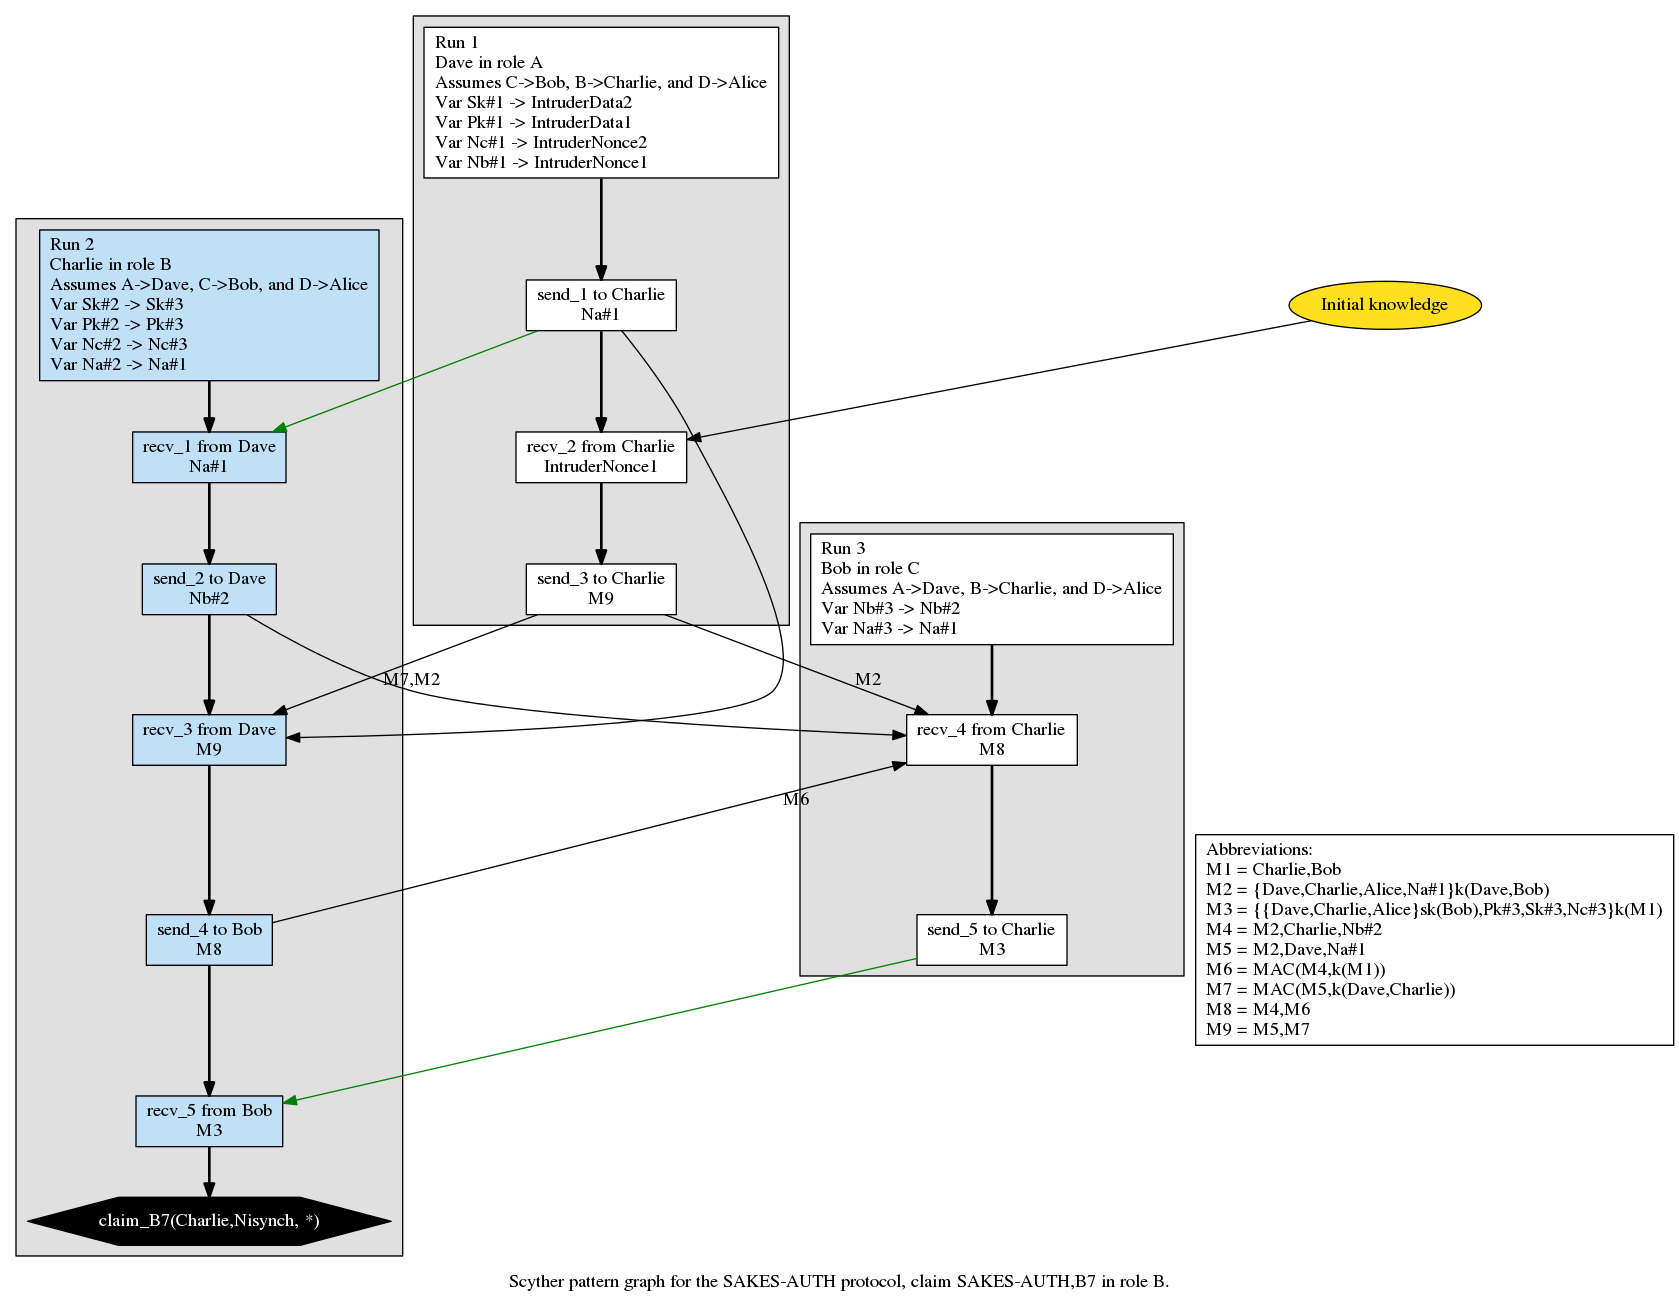
\includegraphics[scale=0.30]{attacks/sakes-auth-a-nisynch-attack2.png}
	\caption{Graph of the attack discovered on the Nisynch property of the roles A, B, and C from A's point of view in the authentication phase of SAKES.}
	\label{fig:sakes-attack-nisynch}
\end{sidewaysfigure}

\begin{sidewaysfigure}
	\centering
	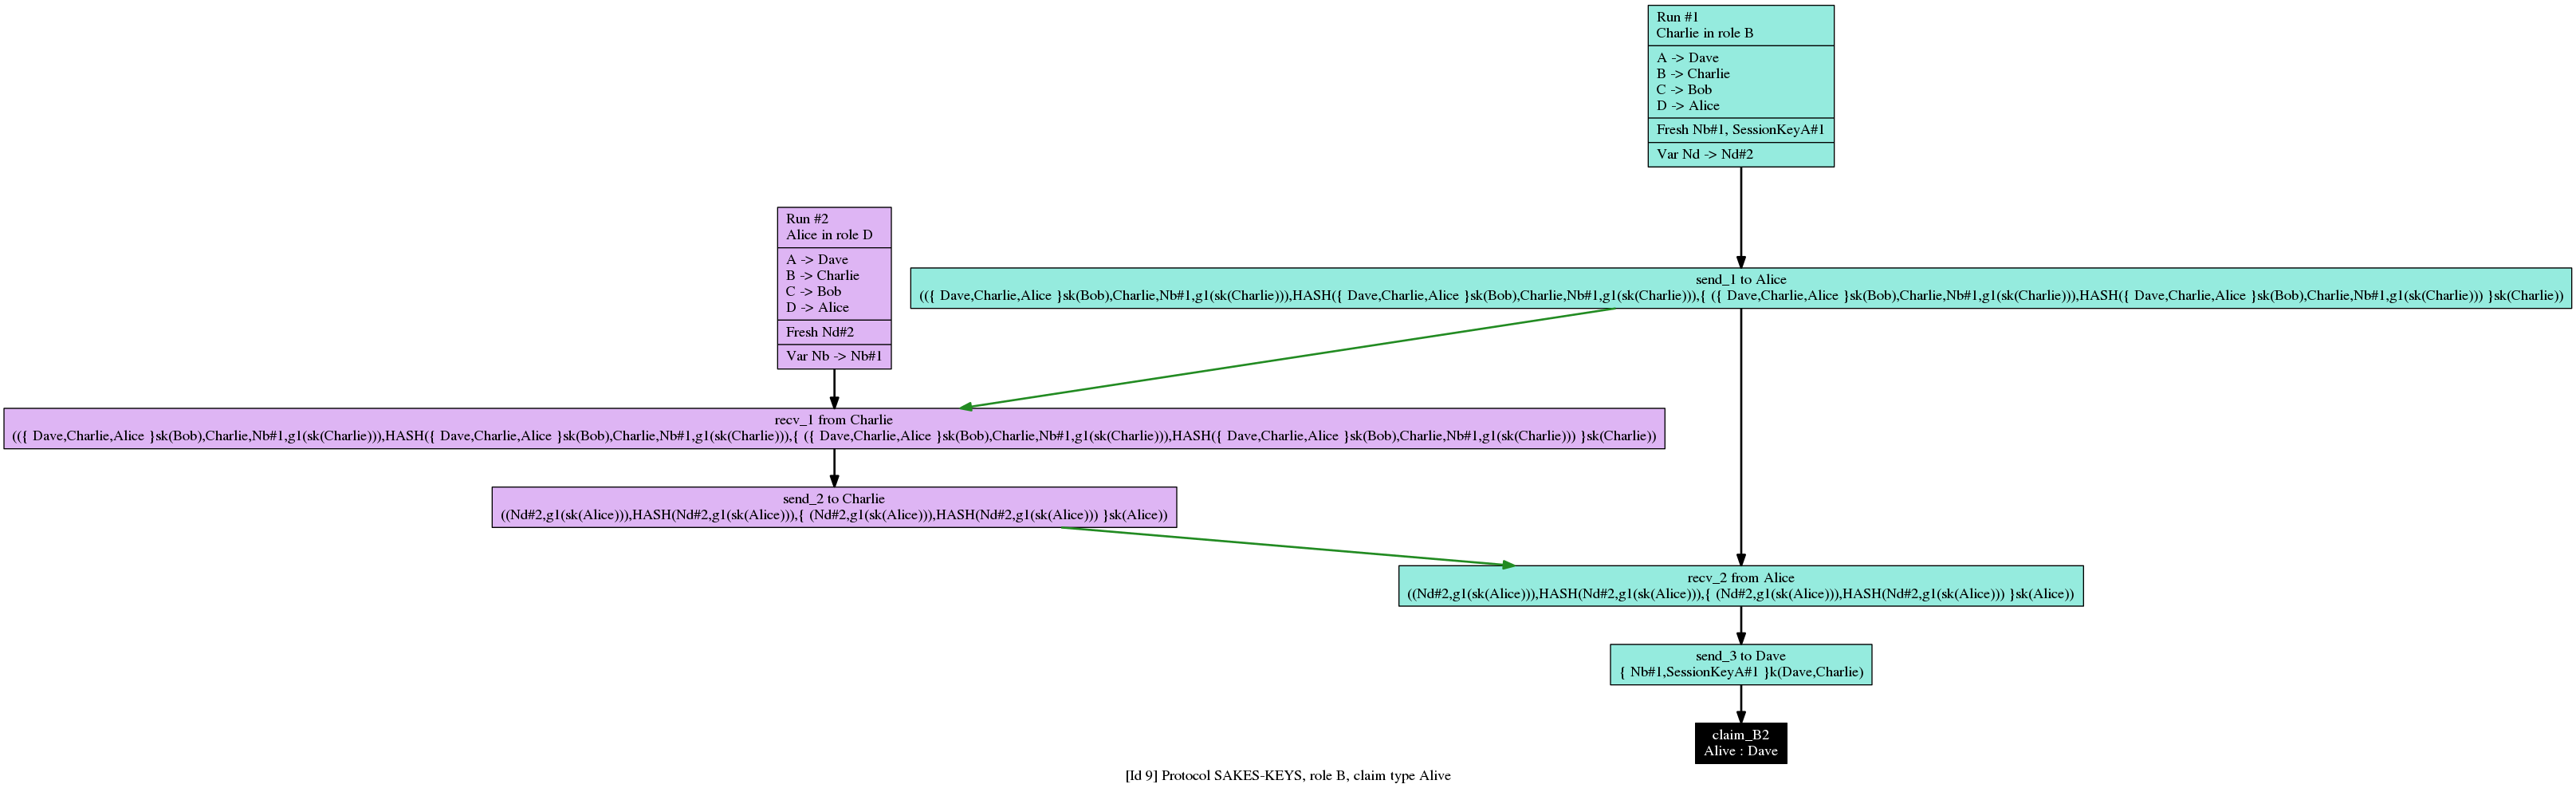
\includegraphics[scale=0.19]{attacks/sakes-keys-b-alive-a-attack.png}
	\caption{Graph of the attack discovered on the entity authentication of the end device in role B in the key establishment phase of SAKES.}
	\label{fig:sakes-attack-keys-b-alive-a}
\end{sidewaysfigure}

\begin{sidewaysfigure}
	\centering
	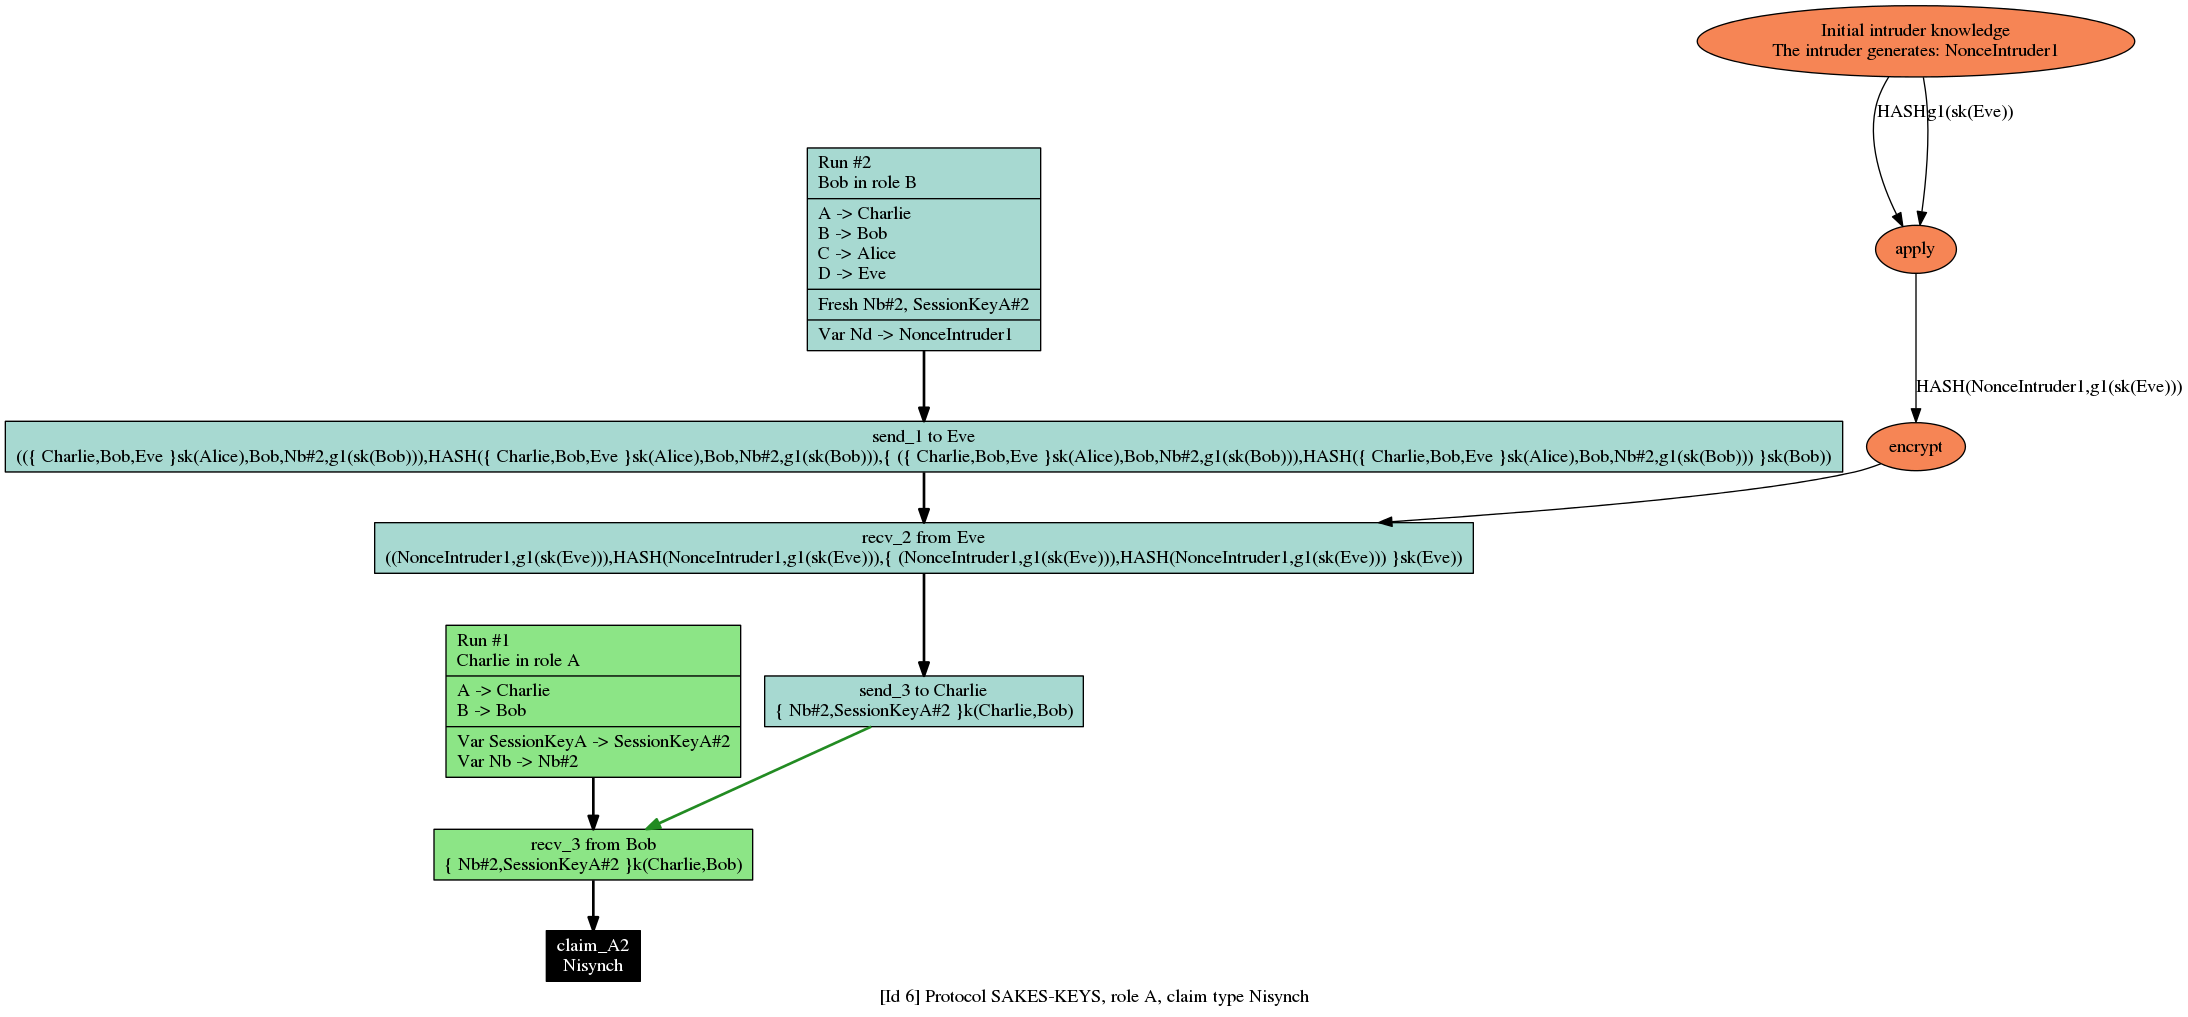
\includegraphics[scale=0.27]{attacks/sakes-keys-a-niagree-nisynch-attack.png}
	\caption{Graph of the attack discovered on the Niagree and Nisynch properties in the role A in the key establishment phase of SAKES.}
	\label{fig:sakes-attack-keys-a-niagree-nisynch}
\end{sidewaysfigure}

\begin{sidewaysfigure}
	\centering
	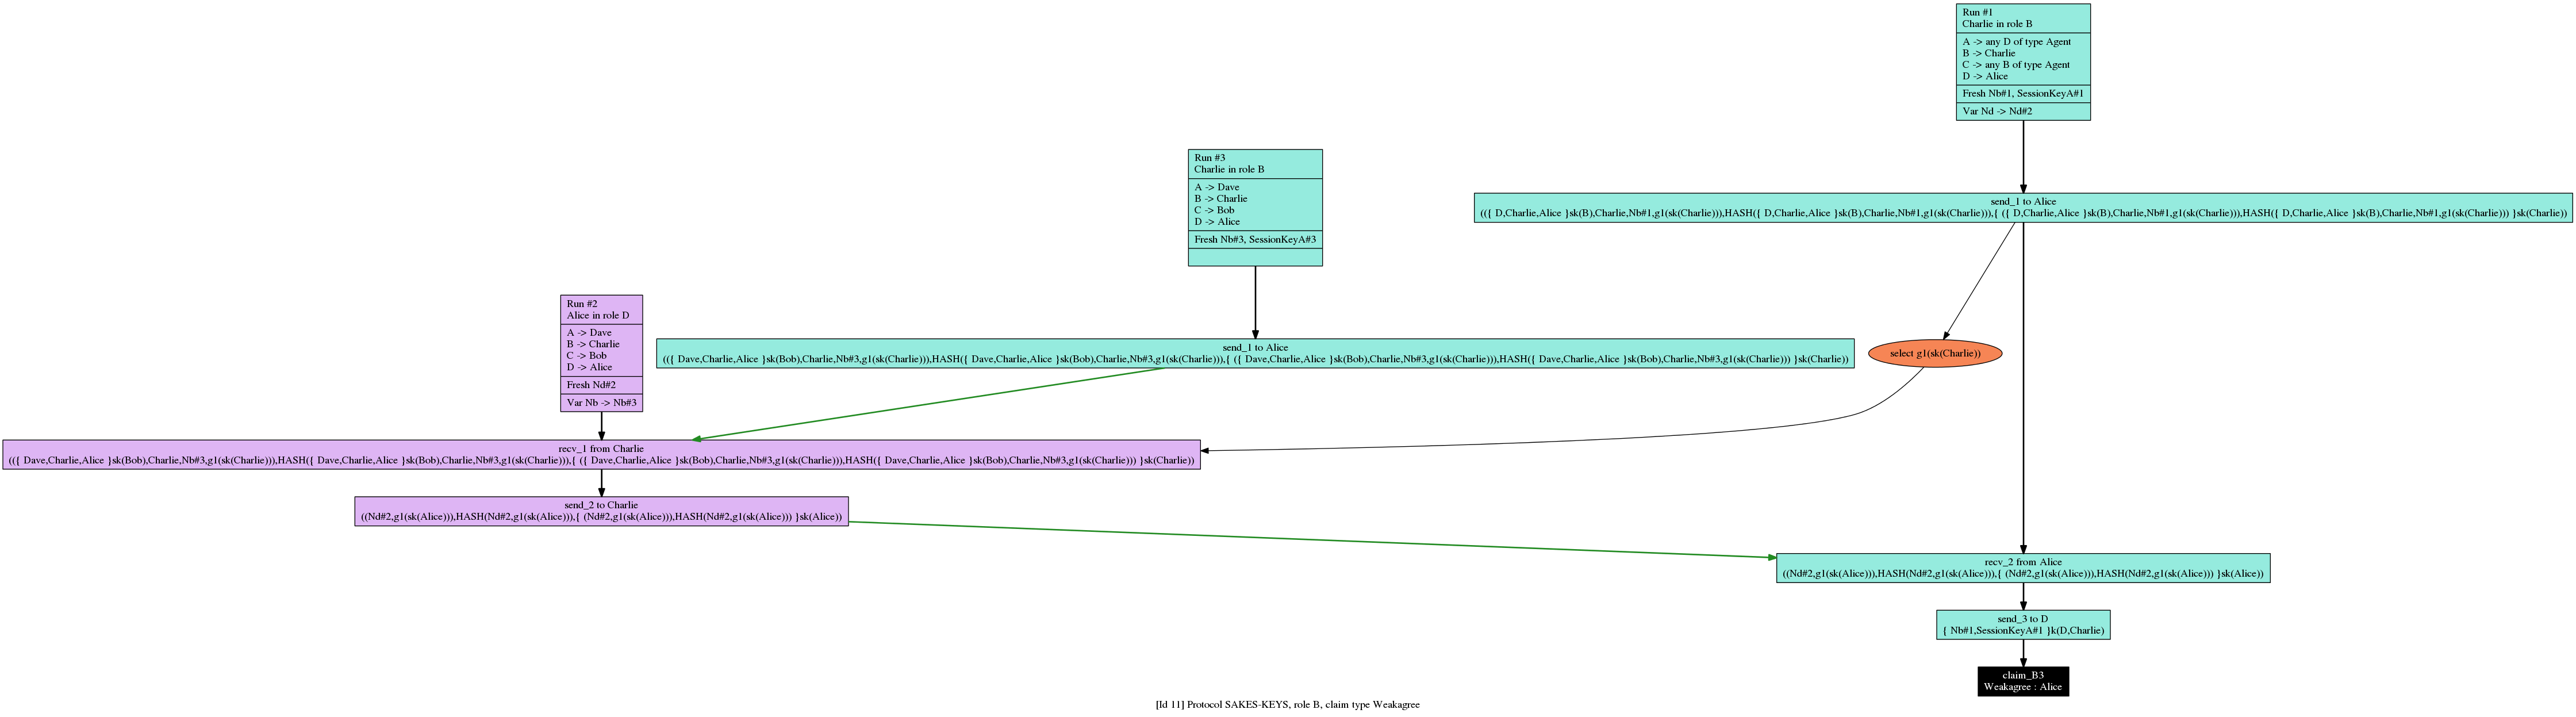
\includegraphics[scale=0.13]{attacks/sakes-keys-b-weakagree-d-attack.png}
	\caption{Graph of the attack discovered on the weakagree property of D in role B in the key establishment phase of SAKES.}
	\label{fig:sakes-attack-keys-b-weakagree-d}
\end{sidewaysfigure}

\begin{sidewaysfigure}
	\centering
	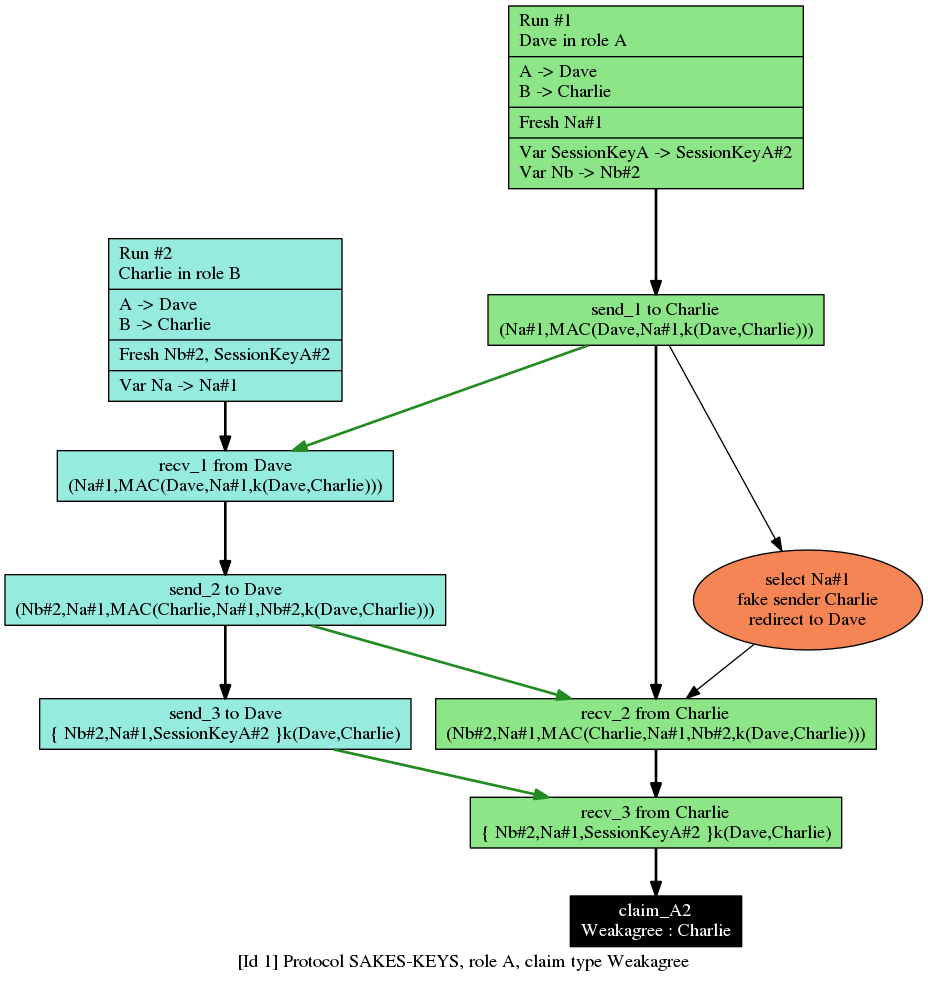
\includegraphics[scale=0.35]{attacks/sakes-keys-a-weakagree-b-attack.png}
	\caption{Graph of the attack discovered on the weakagree property of B in role A in the key establishment phase of SAKES.}
	\label{fig:sakes-attack-keys-a-weakagree-b}
\end{sidewaysfigure}


\chapter{Notations}

\section{Notations}
\label{app:notations}

\begin{tcolorbox}[title=Notations used in protocol specifications]
\begin{tabular}{ll}
\multicolumn{1}{p{1.3cm}}{\textbf{Symbol}} & \multicolumn{1}{p{4cm}}{\textbf{Meaning}}\\
A, B, C, D & Nodes\ A, B, C, D\\
$\langle{\ ...\ }\rangle{}$ & Unauthenticated message\\
$\langle{\ ...\ }\rangle{k}$ & Authenticated message with key $k$\\
$\{\ ...\ \}_k$ & Message encrypted with key $k$\\
$A \rightarrow B$ & Message sent from A to B\\
$A \rightarrow *$ & Message broadcasted from A\\
$(Pk_{node}, Sk_{node})$ & Public key pair for a node \\
$ID_{node}$ & Identity of a node\\
$AES(k, m)$ & AES encryption of message $m$ with key $k$\\
$N_{node}$ & Cryptographic nonce generated by a node\\
$X\ ||\ Y$ & Concatenation of two terms X and Y\\ 
\end{tabular}
\end{tcolorbox}


